% Adapted from https://www.overleaf.com/latex/templates/cse-3500-algorithms-and-complexity-homework-template/wrfwdhfzpnqc

\documentclass[12pt,letterpaper]{article}
\usepackage{fullpage}
\usepackage[top=2cm, bottom=4.5cm, left=2cm, right=2cm]{geometry}
\usepackage{fancyhdr} % Fancy headers
\usepackage{graphicx}
\usepackage{subcaption} % Subfigures
\usepackage{amsmath}
\usepackage{amssymb}
\usepackage{listings}
\usepackage{xcolor}
\usepackage{enumerate}
\usepackage{siunitx}
\usepackage{multicol}
\usepackage{hyperref}
\usepackage{float}
\usepackage{cite}
\usepackage[natbibapa]{apacite} 
\bibliographystyle{apacite}

\setlength{\columnsep}{1cm}

% Edit these as appropriate
\newcommand\course{FIT3179}
\newcommand\hwtitle{Data Visualisation \#2}
\newcommand\nameIDa{Christopher Hall}
\newcommand\nameIDb{3056 5693 / chal0005}

\pagestyle{fancyplain}
\headheight 35pt
\lhead{\nameIDa\\\nameIDb}
\chead{\textbf{\Large \hwtitle}}
\rhead{\course\\\today}
\lfoot{}
\cfoot{}
\rfoot{\small\thepage}
\headsep 1.5em

\hypersetup{
    colorlinks=true,
    linkcolor=blue,
    filecolor=magenta,      
    urlcolor=blue,
    citecolor=blue,
    pdftitle={\hwtitle},
    pdfpagemode=FullScreen,
}

\begin{document}

\begin{titlepage}

    \begin{center}
        \textbf{\LARGE \course} \\
        \vspace{1cm}
        \textbf{\LARGE \hwtitle} \\
        \vspace{3cm}
        \nameIDa \\
        \vspace{3cm}
        Word count: 981 \\
        Link to visualisation: \href{https://hallgchris.github.io/fit3179-dv2}{https://hallgchris.github.io/fit3179-dv2/} \\
        Link to source code: \href{https://github.com/hallgchris/fit3179-dv2}{https://github.com/hallgchris/fit3179-dv2}
    \end{center}

\end{titlepage}


\begin{multicols}{2}


    \section*{Introduction}

    In my visualisation, I explore patterns and correlations in the installation of photovoltaic or ``solar'' panels in Australia. This visualisation doesn't serve a technical purpose - rather, it aims to educate and satisfy a curiosity in the average Australian resident, especially those who may have noticed and wondered why solar panels are more common in some places than others.

    \section*{What}

    All of my solar-related data came originated from~\citep{noauthor_australian_2022}. This came as several tabular (csv) datasets including a breakdown of solar usage by Local Government Area (LGA) and monthly solar installations/capacity data. This data is already aggregated primarily but not solely from~\citep{noauthor_postcode_2022}, which proves useful as data not inherently related to solar (but relevant to the visualisation) is present in the dataset.

    Geographical information (specifically LGA and state boundary locations and names) were sourced from~\citep{noauthor_digital_nodate}.

    I then used several python scripts to perform simple operations including merging multiple CSVs with slightly differing formats, reducing the number of ordinal data types (by merging smaller ones into larger ones), and aggregating state data into national. These scripts, like the rest of the visualisation code, can be viewed on \href{https://github.com/hallgchris/fit3179-dv2}{GitHub}.

    \section*{Why and how}

    An image of the entire visualisation is attached in the appendix.

    \subsection*{Choropleth map}

    \begin{figure}[H]
        \centering
        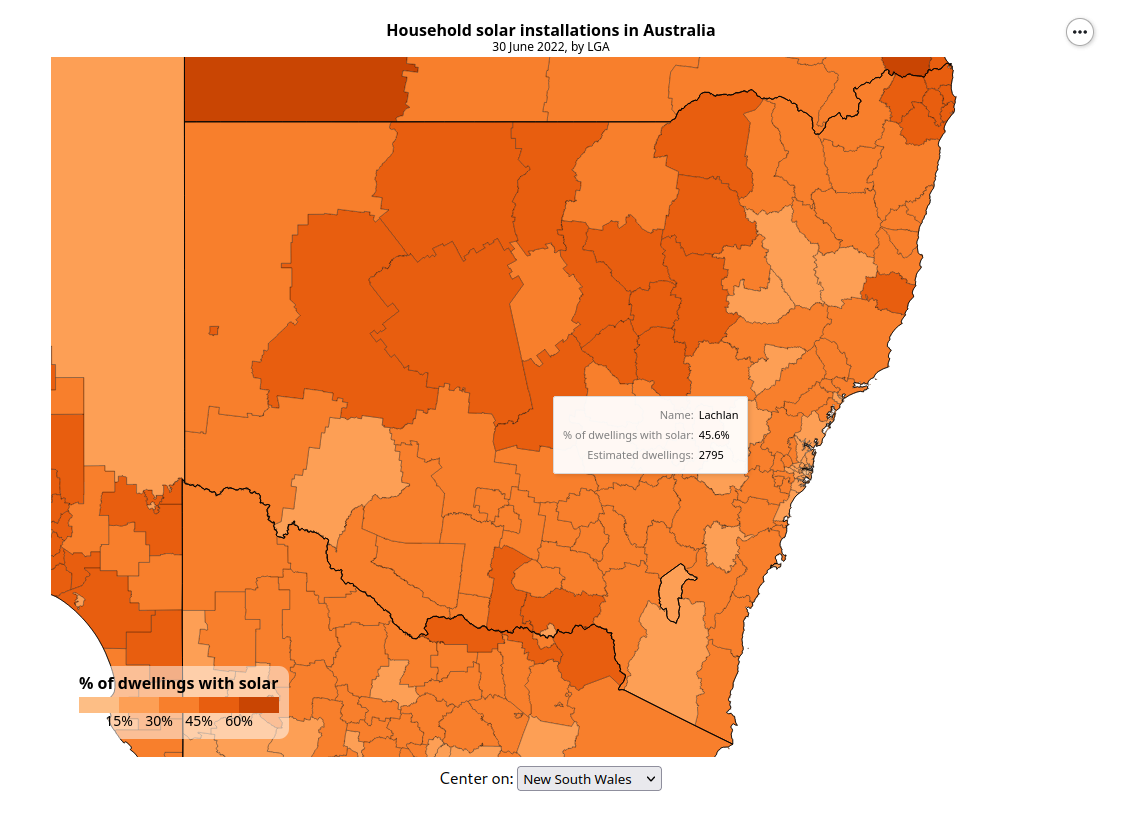
\includegraphics[width=\linewidth]{images/map.png}
        \caption{The choropleth map as shown in the visualisation.}
        \label{fig:map}
    \end{figure}

    The choropleth map (figure~\ref{fig:map}) is a familiar and intuitive idiom providing a familiar invitation to the viewer to read the visualisation.

    A choropleth map was the best choice of idiom to display this data. We could compare to a dot density map, for example - dot density is well suited to showing the locations of discrete points of interest, but here we only have one point per LGA representing an average across the respective area. Hence, it makes sense to have a mark that reflects that the whole area is relevant.

    The state-level zoom provides enough detail to resolve the smallest LGAs in populous CBDs, while the national-level zoom provides an effective overview of the country enabling large-scale trends to be observed.

    \subsection*{Heatmap}

    \begin{figure}[H]
        \centering
        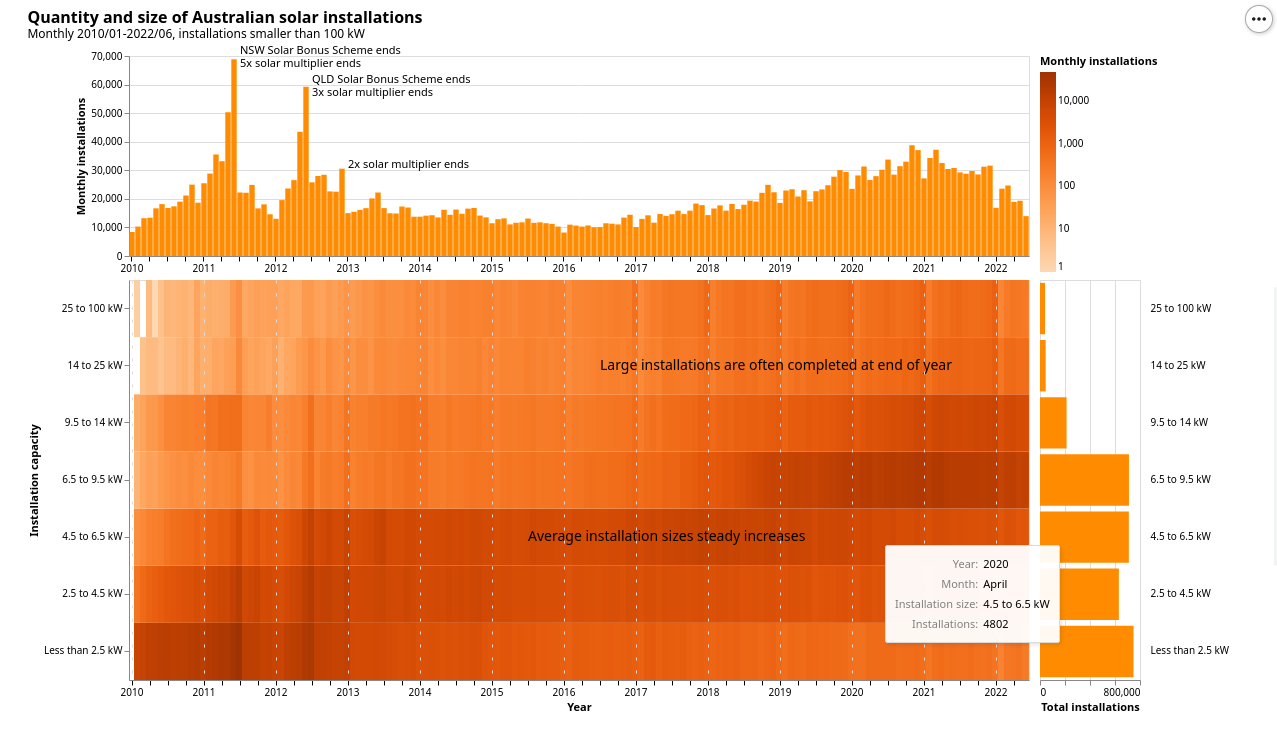
\includegraphics[width=\linewidth]{images/heatmap.png}
        \caption{The heatmap with histograms as shown in the visualisation.}
        \label{fig:heatmap}
    \end{figure}

    This is easily the most complex idiom of this visualisation.

    The heatmap (figure~\ref{fig:heatmap}) is a great choice as it lets me encode two ordinal data channels (in this case installation size and month) while clearly showing their nominal order. For comparison, an inferior alternative would be a line chart with an ordinal channel encoded in colour hue and/or value. This was attempted by APVI, copied here in figure~\ref{fig:apvi-line}.

    \begin{figure}[H]
        \centering
        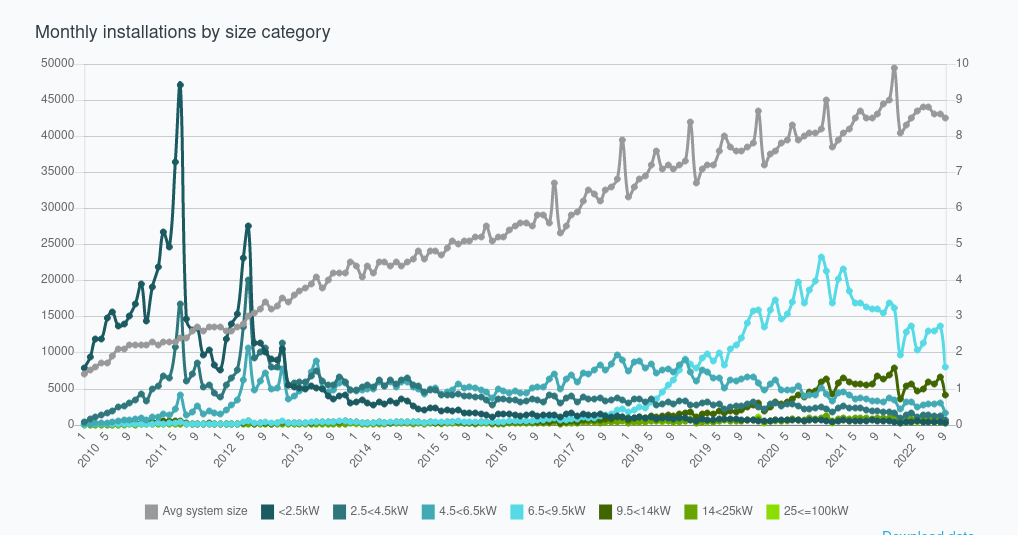
\includegraphics[width=\linewidth]{images/apvi-line.png}
        \caption{APVI's line chart visualisation of the same data. Sourced from \href{https://pv-map.apvi.org.au/analyses}{APVI}. \cite{noauthor_australian_2022}}
        \label{fig:apvi-line}
    \end{figure}

    Compared to my visualisation (figure~\ref{fig:heatmap}), the nature of the line chart means that lines obscure each other, and it is hard to tell which line should come "after" another in the installation capacity channel. This is not an issue in the heatmap.

    Another issue with the APVI visualisation is the requirement of a second y-axis to show the increasing average system size. This is not ideal as it is not clear which lines should use which axis. In the heatmap, the trend of increasing installation size is visible without even being explicitly displayed.

    A potential issue with the heatmap is that on its own it does not show "totals". This is solved with the histograms above and beside the heatmap, which concisely show how installations change when either ordinal channel is ignored. This again would not be possible with the line chart idiom.

    \subsection*{Normalised bar chart}

    \begin{figure}[H]
        \centering
        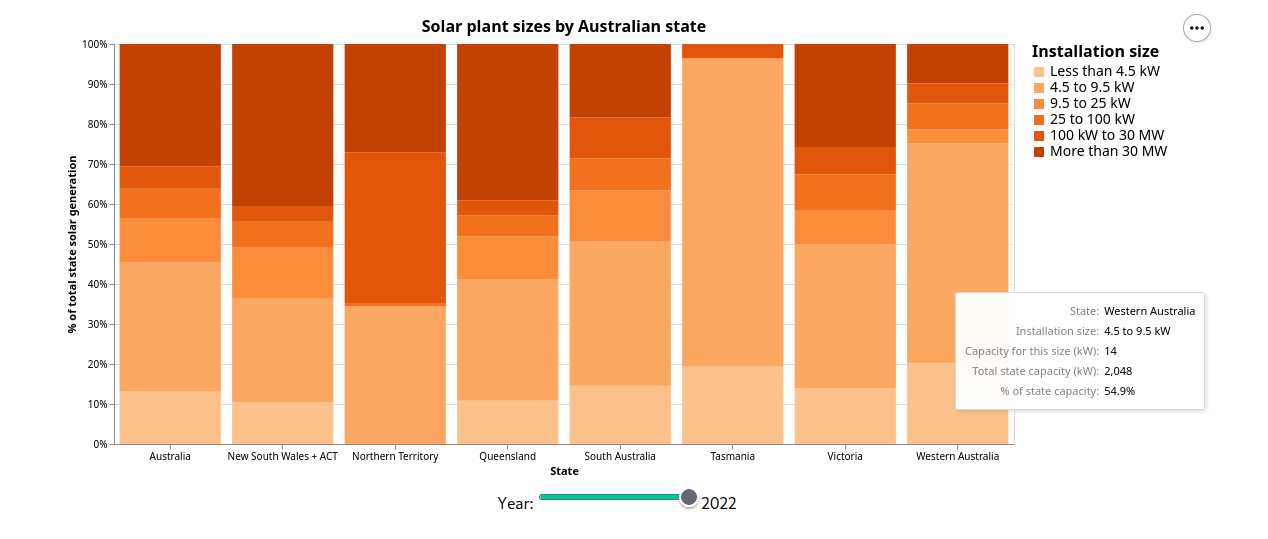
\includegraphics[width=\linewidth]{images/bar.png}
        \caption{The normalised bar chart as shown in the visualisation.}
        \label{fig:bar}
    \end{figure}

    Normalising the bar chart (figure~\ref{fig:bar}) is a requirement due to the large range of solar generation capabilities between states. Were this not done, it would be impossible to see the different coloured sections of the smaller bars. It's the composition of the solar generation that we're interested in here, not the magnitude (which is explored in the next section).

    The time channel is adjusted with a slider rather than being encoded in the visualisation. This is because while change over time is interesting, it provides less insight into Australian solar compared to other channels when considering the other time-series visualisations available elsewhere on the page. So, it is treated as an "extra" that the viewer may choose to explore.

    \subsection*{Line chart}

    \begin{figure}[H]
        \centering
        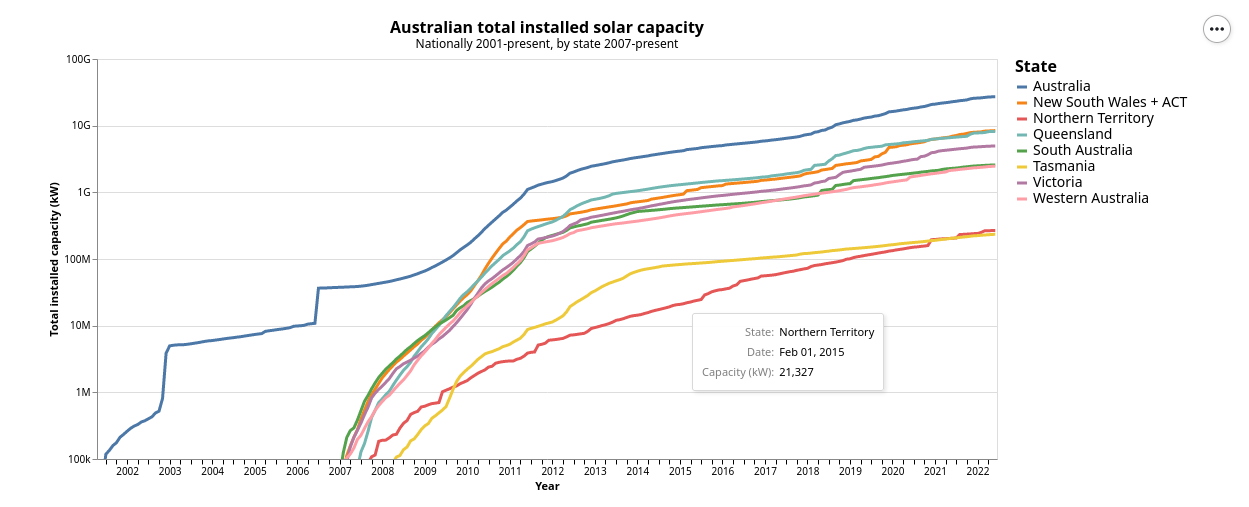
\includegraphics[width=\linewidth]{images/line.png}
        \caption{The logarithmic line chart as shown in the visualisation.}
        \label{fig:line}
    \end{figure}

    A line chart (figure~\ref{fig:line}) is a nice simple idiom where a log scale is easily used for displaying the exponential growth of Australia's solar generation without compromising on detail at any point.

    \section*{Design}

    \subsection*{Layout}

    At most screen resolutions, the body text is split into 3 columns in order to restrict line length, improving readability. On narrow screens it collapses onto a single column, and on wide screens the maximum width is capped, for the same reason.

    Charts in Vega Lite are difficult to make responsive to UI resizing, and since it's beyond the scope of this unit I've not gone to the effort. Instead, I've chosen a fixed (equal) width which works on most screen sizes and fits all the data well.

    \begin{figure}[H]
        \centering
        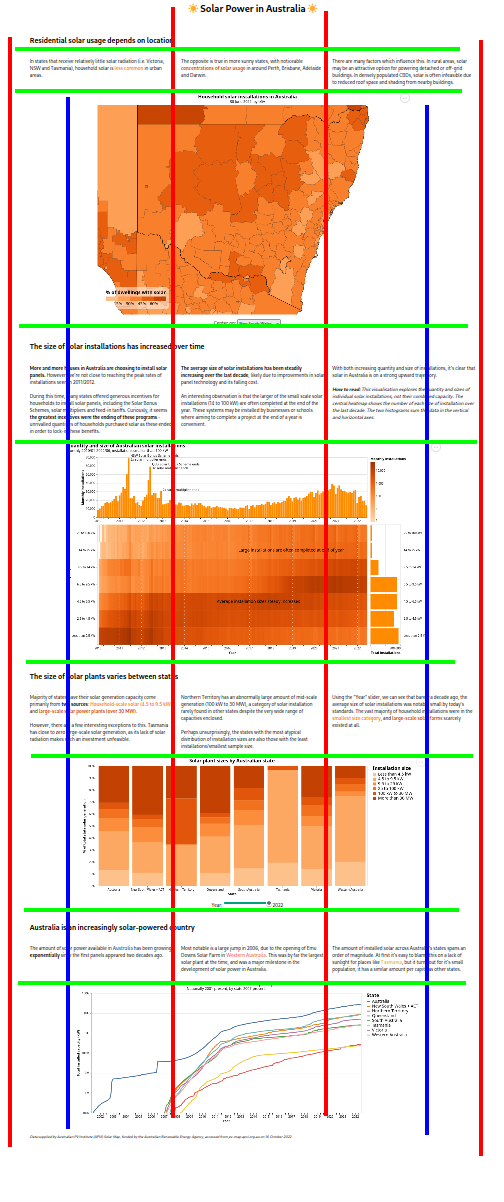
\includegraphics[width=0.9\linewidth]{images/sight.png}
        \caption{The sight lines in the visualisation. Red/green lines are between text, blue/green lines are between visualisations.}
        \label{fig:sight}
    \end{figure}

    Whatever the screen size, there will always be sight lines between the titles and text paragraphs, and separate lines between the visualisations, annotated in figure~\ref{fig:sight}.

    The paragraphs and visualisations are centred on screen, providing visual balance to the page.

    \subsection*{Colour}

    Black text on a white background is used for readability.

    Visualisations use a single-hue orange colour palette to encode data, reflecting the warmth of sunlight associated with solar energy. Between charts, the same orange colour encodes slightly different attributes, but I believe it is justified as in all cases it encodes the degree to which solar is used and darker approximately means "more solar".

    Where possible, words in text were coloured with an appropriate colour from the visualisation.

    \subsection*{Figure-ground}

    Titles and key phrases are emphasised using font weight and size.

    \subsection*{Typography}

    A generic sans-serif font, in my case ``Cantarell'', is selected and used throughout the visualisation. This provides easy-to-read text and a clean, modern look. As discussed, columns, font weight and font size are used effectively.

    \subsection*{Storytelling}

    The visualisation is vertically oriented (as are most websites) so that the intended order of reading is obvious.

    Columns are separated by visualisations so it is never ambiguous whether to read down or across.

    Visualisations are accompanied by concise but informative interpretations and insights into the data being displayed.

    \bibliography{dv2_report}{}

\end{multicols}

\end{document}

